\documentclass[conference]{IEEEtran}
\IEEEoverridecommandlockouts
% The preceding line is only needed to identify funding in the first footnote. If that is unneeded, please comment it out.
\usepackage{comment}
\usepackage{caption}
\usepackage{subcaption}
\usepackage{hyperref}
\usepackage{floatrow}
\usepackage{cite}
\usepackage{amsmath,amssymb,amsfonts}
\usepackage{algorithmic}
\usepackage{graphicx}
\usepackage{textcomp}
\usepackage{xcolor}
\def\BibTeX{{\rm B\kern-.05em{\sc i\kern-.025em b}\kern-.08em
    T\kern-.1667em\lower.7ex\hbox{E}\kern-.125emX}}
\begin{document}
{\fontfamily{lmss}\selectfont{
\title{Assignment 1 : Basic Image Editor}


% {\footnotesize \textsuperscript{*}Note: Sub-titles are not captured in Xplore and
% should not be used}
% \thanks{Identify applicable funding agency here. If none, delete this.}
% }

\author{\IEEEauthorblockN{Rohit Vartak}
\IEEEauthorblockA{\textit{Department of Electrical Engineering} \\
\textit{190010058}\\
190010058@iitb.ac.in}}

\maketitle

\begin{abstract}
%One paragraph summary of motivation for the study, the gap in existing analyses that your work fills, data sources used, analyses done or methodological innovations, main findings, and main conclusion.
We can perform various operations on our images to extract more  information from them. For example, we can perform log transformations, power law transformations etc. Images are just arrays with three channels for the 3 colors namely R, G and B and hence we can use the numpy class of python to perform operations on the image. We also develop a GUI in python to stream line the process of transformation of the image.
\end{abstract}

\begin{IEEEkeywords}
GUI, image, transformation, 
\end{IEEEkeywords}

\section{Introduction}
%A few paragraphs about the broader problem, the importance of knowing the answer or finding a solution, the specific question that has not been satisfactorily answered in existing analyses, the specific question(s) that your work answers or the specific innovation of your work, the datasets that will help you get your answer, the main ideas behind the experiment or analysis plan, and the metrics that will help you evaluate the results.
%Related work: What similar work or background work has been done on this topic, what were their main ideas, findings, and shortcomings that help to frame the importance or relevance of your work.
The main objective was to perform various operations on images which were taught in class. Since images are at the end of the day just arrays one had to use the vectorization made available to us in python so as to make the operations on the image arrays fast. We perform various operations on our image, for example, we perform Equalize histogram, Gamma correct , Log transform,  Blur with a mechanism to control the extent of blurring and Sharpening with a mechanism to control the extent of sharpening.
\newline We also define the convolution function between two arrays as:
\begin{figure}[htbp]
\centerline{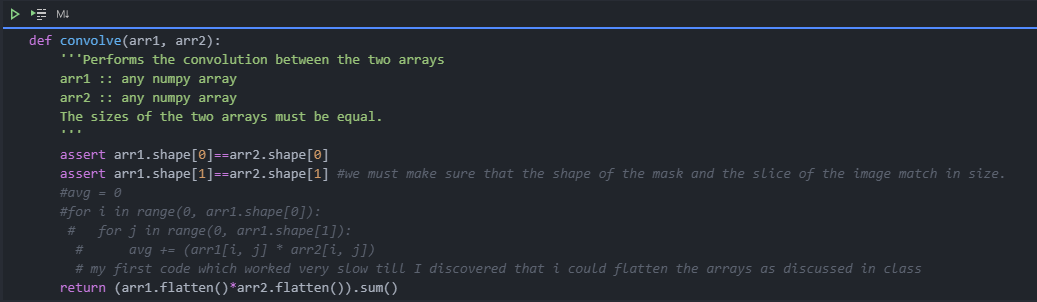
\includegraphics[scale = 0.30]{images/convolve.png}}
\caption{Convolution}
\label{fig:gui_1}
\end{figure}
We can first flatten each array and then  multiply and add ,which is much faster than doing it with 2 for loops and element wise multiplication.
\section{ GUI design}

I used tkinter from python to implement the GUI features of the assignment.
I have been able to implement the following features in the gui:
\begin{enumerate}
    \item  Image display area
    \item  Image load button that opens a file selector
    \item Manipulate buttons for the following operations:
    \begin{itemize}
        \item  Equalize histogram
        \item Gamma correct (ask for input gamma upon pressing the button)
        \item Log transform
        \item Blur with a mechanism to control the extent of blurring
        \item Sharpening with a mechanism to control the extent of sharpening
    \end{itemize}
\end{enumerate}
\begin{figure}[htbp]
\centerline{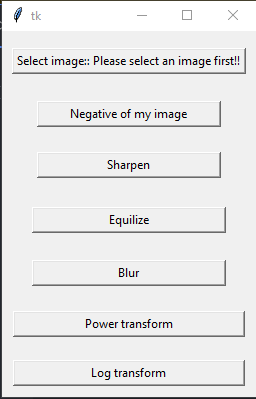
\includegraphics[scale = 0.50]{images/gui.png}}
\caption{GUI looks}
\label{fig:gui_1}
\end{figure}
\begin{figure}[htbp]
\centerline{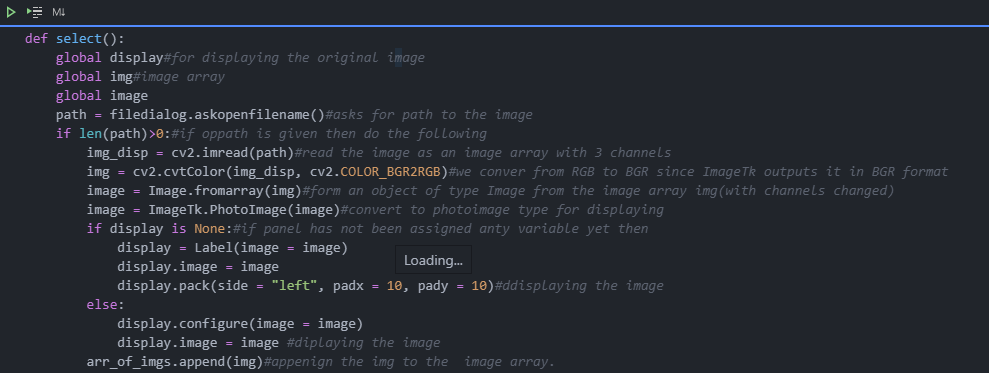
\includegraphics[scale = 0.30]{images/select.png}}
\caption{Image selection block}
\label{fig:gui_1}
\end{figure}
\begin{figure}[htbp]
\centerline{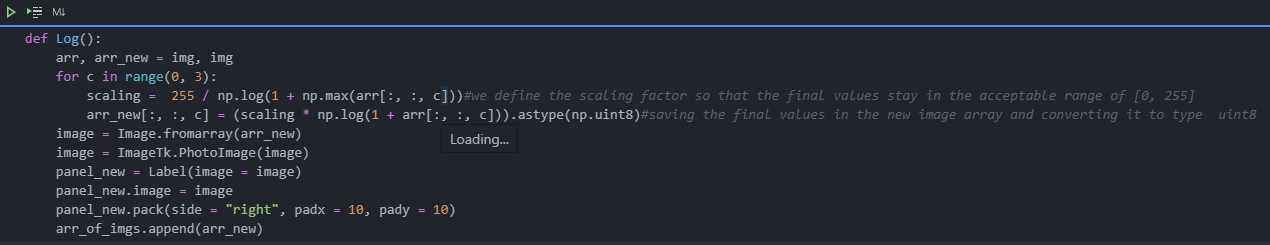
\includegraphics[scale = 0.25]{images/log_gui.png}}
\caption{Log transform block}
\label{fig:gui_1}
\end{figure}
\begin{figure}[htbp]
\centerline{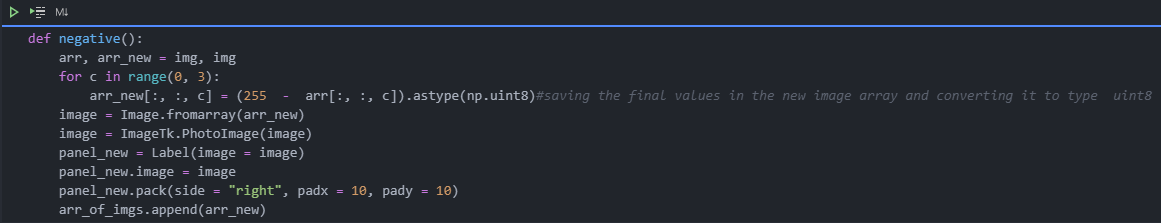
\includegraphics[scale = 0.30]{images/neg_gui.png}}
\caption{Negative of an image block}
\label{fig:gui_1}
\end{figure}
\begin{figure}[htbp]
\centerline{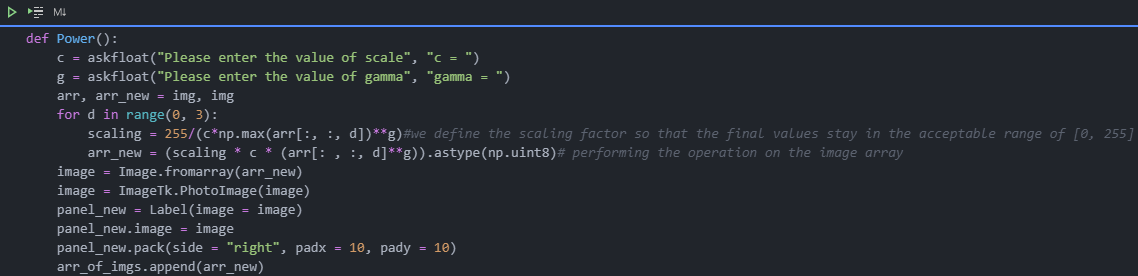
\includegraphics[scale = 0.30]{images/power_gui.png}}
\caption{Gamma correction block}
\label{fig:gui_1}
\end{figure}
\begin{figure}[htbp]
\centerline{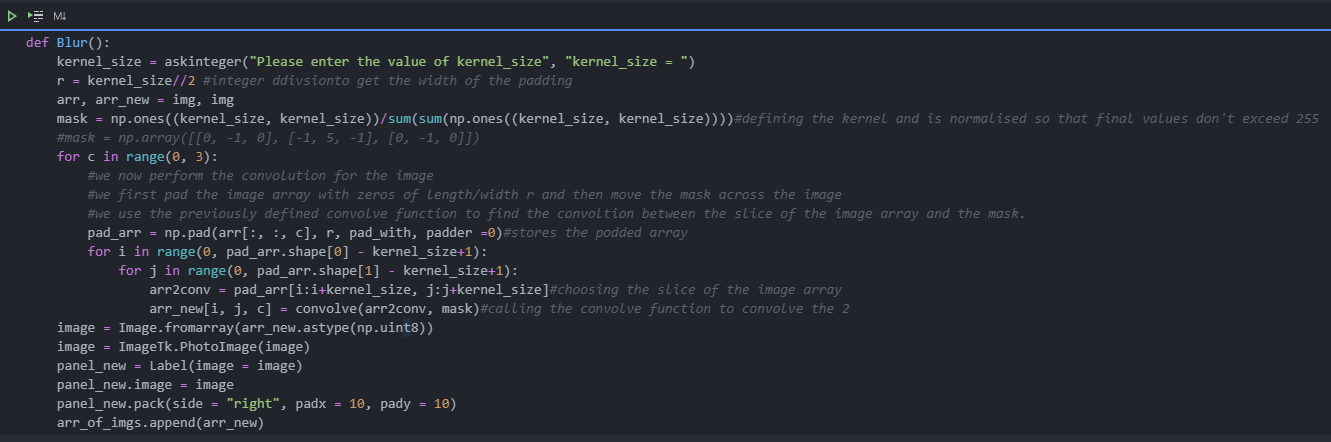
\includegraphics[scale = 0.25]{images/blur_gui.png}}
\caption{Blurring block}
\label{fig:gui_1}
\end{figure}
\begin{figure}[htbp]
\centerline{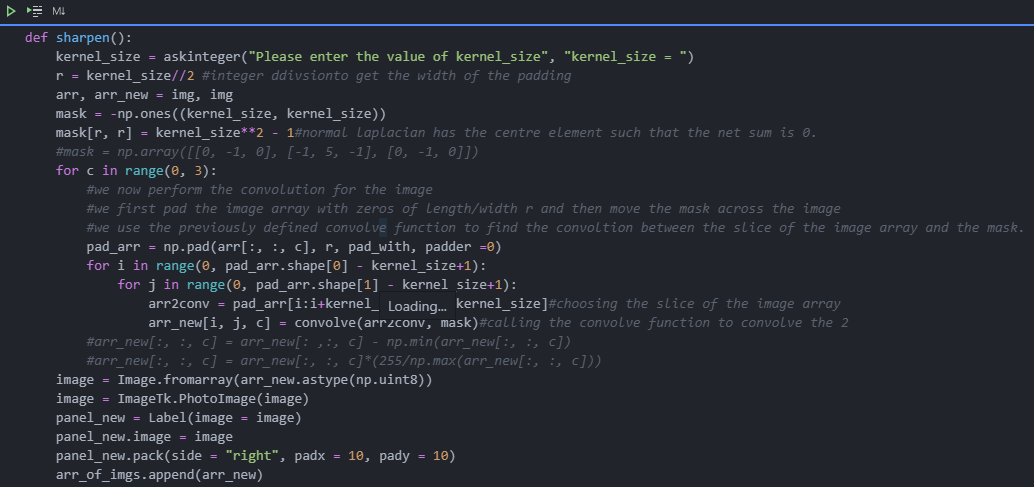
\includegraphics[scale = 0.30]{images/sharpen_gui.png}}
\caption{Sharpen image block}
\label{fig:gui_1}
\end{figure}
\begin{figure}[htbp]
\centerline{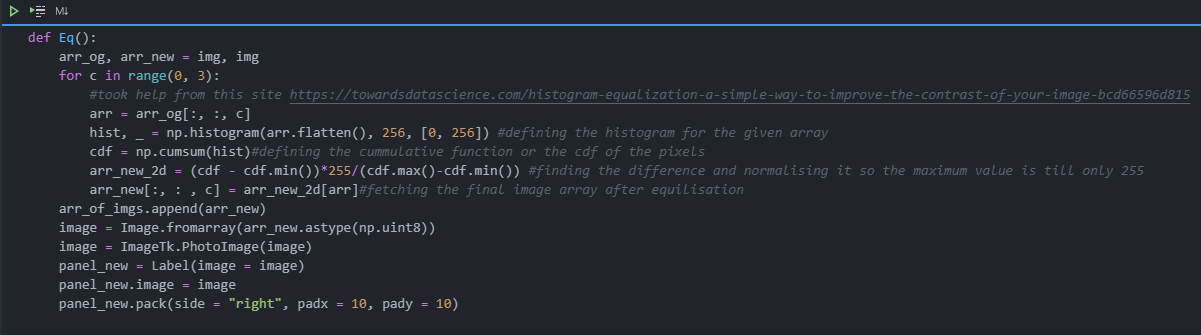
\includegraphics[scale = 0.30]{images/eq_gui.png}}
\caption{Historgram equilisation block}
\label{fig:gui_1}
\end{figure}
%\subsection{Maintaining the Integrity of the Specifications}

%The IEEEtran class file is used to format your paper and style the text. All margins, 
%column widths, line spaces, and text fonts are prescribed; please do not 
%alter them. You may note peculiarities. For example, the head margin
%measures proportionately more than is customary. This measurement 
%and others are deliberate, using specifications that anticipate your paper 
%as one part of the entire proceedings, and not as an independent document. 
%Please do not revise any of the current designations.

%A summary paragraph of data requirements, a few paragraphs about each data source, their organization, fields, and values, their issues, how they can be merged or cleaned, and some tables showing sample entries in each data source, or summarizing the data sources at a high level.

\section{Image Processing}
%Before you begin to format your paper, first write and save the content as a 
%separate text file. Complete all content and organizational editing before 
%formatting. Please note sections \ref{AA}--\ref{SCM} below for more information on 
%proofreading, spelling and grammar.

%Keep your text and graphic files separate until after the text has been 
%formatted and styled. Do not number text heads---{\LaTeX} will do that 
%for you.

\subsection{Image processing operations implemented}\label{AA}
%Define abbreviations and acronyms the first time they are used in the text, 
%even after they have been defined in the abstract. Abbreviations such as 
%IEEE, SI, MKS, CGS, ac, dc, and rms do not have to be defined. Do not use 
%abbreviations in the title or heads unless they are unavoidable.
We have implemented the following image processes- 
\begin{itemize}
    \item Equalize histogram
    \item Gamma correct
    \item Log transform
    \item  Blur with a mechanism to control the extent of blurring 
    \item Sharpening with a mechanism to control the extent of sharpening
    \item My own feature : Image negative
\end{itemize}
\subsection{Purpose of the above transformations}

%\begin{itemize}
%\item Use either SI (MKS) or CGS as primary units. (SI units are encouraged.) English units may be used as secondary units (in parentheses). An exception would be the use of English units as identifiers in trade, such as ``3.5-inch disk drive''.
%\item Avoid combining SI and CGS units, such as current in amperes and magnetic field in oersteds. This often leads to confusion because equations do not balance dimensionally. If you must use mixed units, clearly state the units for each quantity that you use in an equation.
%\item Do not mix complete spellings and abbreviations of units: ``Wb/m\textsuperscript{2}'' or ``webers per square meter'', not ``webers/m\textsuperscript{2}''. Spell out units when they appear in text: ``. . . a few henries'', not ``. . . a few H''.
%\item Use a zero before decimal points: ``0.25'', not ``.25''. Use ``cm\textsuperscript{3}'', not ``cc''.)
%\end{itemize}
\begin{itemize}
    \item \textit{Equalize histogram} : Helps in improving the contrast of the image.
    \item \textit{Gamma correct} :  It controls the overall brightness of an image.
    \item \textit{Log transform} :  Log transformation is used for image enhancement as it expands dark pixels of the image as compared to higher pixel values.(since the function is convex in nature.)
    \item  \textit{Blur with a mechanism to control the extent of blur} : Helps in reducing the noise of the image and also reduce the details of the image. 
    \item \textit{Sharpening with a mechanism to control the extent of sharpening} : helps in finding the fine details in an image.
\end{itemize}
\subsection{Mathematical formulae}
%Number equations consecutively. To make your 
%equations more compact, you may use the solidus (~/~), the exp function, or 
%appropriate exponents. Italicize Roman symbols for quantities and variables, 
%but not Greek symbols. Use a long dash rather than a hyphen for a minus 
%sign. Punctuate equations with commas or periods when they are part of a 
%sentence, as in:
%\begin{equation}
%a+b=\gamma\label{eq}
%\end{equation}

%Be sure that the 
%symbols in your equation have been defined before or immediately following 
%the equation. Use ``\eqref{eq}'', not ``Eq.~\eqref{eq}'' or ``equation \eqref{eq}'', except at 
%the beginning of a sentence: ``Equation \eqref{eq} is . . .''
\begin{enumerate}

\item \textit{Gamma correct}
\newline Input value of the pixel in the image = $r$
\newline Output value of the pixel in the image = $s$
\begin{equation}
\text{s = T(r) = } c\times r^\gamma\label{eq1}
\end{equation}
Note: We need to normalise the values of the above transformation to ensure that the final values remain within the acceptable limits.\\
%------------------------------------------------------------
\item \textit{log transform}
\newline Input value of the pixel in the image = $r$
\newline Output value of the pixel in the image = $s$
\begin{equation}
\text{s = T(r) = } c\times log(1 + r)\label{eq2}
\end{equation}
Note: We need to normalise the values of the above transformation to ensure that the final values remain within the acceptable limits.
%------------------------------------------------------------
\item \textit{Blurring}\\
For this we use a kernel of all $\frac{1}{(kernel\_size)^2}$.This is done to normalise the kernel, so that the output is always less than 255. Further, we always choose the kernel\_size as an odd integer and pad the image array with the appropriate number of rows and columns.

\item \textit{Sharpening}:\\
For this we use the Laplace filter. This has the value $kernel\_size^2-1$ as the value in the centre and the rest of the value as $-1$. Notice that the elements of this add up to zero and we run the risk of getting a pixel value negative and thus we need to normalise the final values after convolving by subtracting the minimum and then multiplying with $\frac{1}{Max}$.

\item \textit{Negative}\\
\newline Input value of the pixel in the image = $r$
\newline Output value of the pixel in the image = $s$
\begin{equation}
\text{s = T(r) = } 255 - r\label{eq3}
\end{equation}
\end{enumerate}
%------------------------------------------------------------
\section*{Observation and results}
\textbf{NOTE : }\textit{ Since I was not able to implement the save functionality, I am forced to take the screenshots of the output from my GUI. I have provided the images in the .zip file for testing and verification!.}
\begin{enumerate}
    \item \textit{Equalize Histogram} :\\ 
    \begin{figure}[htbp]
\centerline{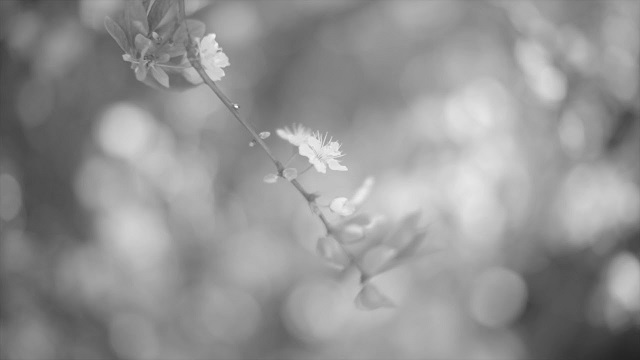
\includegraphics[scale = 0.30]{images/hist.jpeg}}
\caption{Before histogram equilization}
\label{fig:hist_eq_1}
\end{figure}
    \begin{figure}[htbp]
\centerline{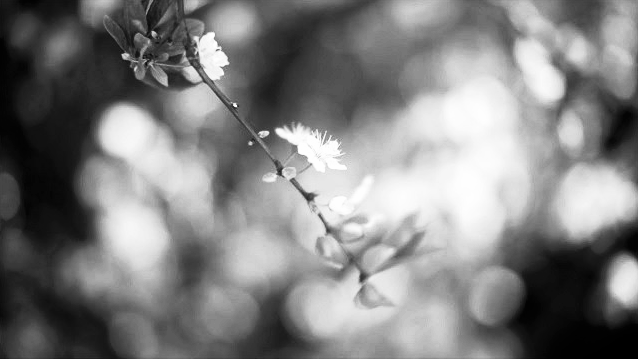
\includegraphics[scale = 0.30]{images/hist_out.png}}
\caption{After histogram equilization}
\label{fig:hist_eq_2}
\end{figure}
\newline Refer to Figure(\ref{fig:hist_eq_1}) and (\ref{fig:hist_eq_2}).Thus, we notice that the latter image has better contrast, i.e it has pixels which are lighter and darker than the original image and this is due to histogram equilisation.
\item \textit{Gamma correct} :\\
 We take the following image: Refer Figures(\ref{fig:gamma_1} and \ref{fig:gamma_2})
     \begin{figure}[htbp]
\centerline{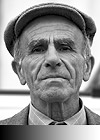
\includegraphics[scale = 1]{images/gamma.jpg}}
\caption{Before gamma correct}
\label{fig:gamma_1}
\end{figure}
    \begin{figure}[htbp]
\centerline{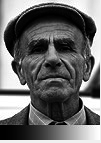
\includegraphics[scale = 1.3]{images/gamma_out.png}}
\caption{After gamma correct}
\label{fig:gamma_2}
\end{figure}
\newline Since $\gamma = 2$, we see that the lighter pixels have been mapped to the darker ones and hence we observe a much darker image for $\gamma >1$.(referring to figures \ref{fig:gamma_1} and \ref{fig:gamma_2})
\item \textit{Log transformation} : \\
 We take the following image: Refer Figures(\ref{fig:log_1} and \ref{fig:log_2})
     \begin{figure}[htbp]
\centerline{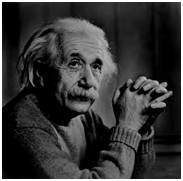
\includegraphics[scale = 0.5]{images/log.jpg}}
\caption{Before log transformation}
\label{fig:log_1}
\end{figure}
    \begin{figure}[htbp]
\centerline{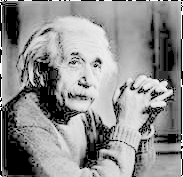
\includegraphics[scale = 0.67]{images/log_out.png}}
\caption{After log transformation}
\label{fig:log_2}
\end{figure}
\newline Thus, since log is convex function we observe that the darker pixels are expanded out while the lighter ones are mapped over a larger range. Thus, we end up compressing the higher pixel values.
\item \textit{Blurring} :\\ 
 We take the following image: 
     \begin{figure}[htbp]
\centerline{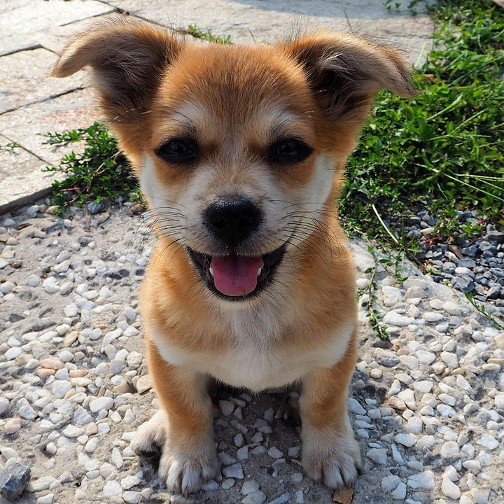
\includegraphics[scale = 0.5]{images/doggo.jpeg}}
\caption{Before blurring}
\label{fig:blur_1}
\end{figure}
    \begin{figure}[htbp]
\centerline{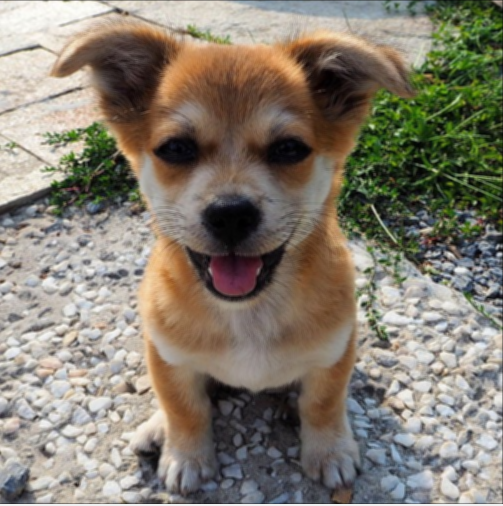
\includegraphics[scale = 0.67]{images/blur_out.png}}
\caption{After blurring}
\label{fig:blur_2}
\end{figure}
\newline Referring to Figures (\ref{fig:blur_1}) and (\ref{fig:blur_2}), we choose a $3\times 3$ kernel size for our blurriing.
\item \textit{The feature I have added : Negative of an Image} : \\
Taking the negative of the image from Figure(\ref{fig:log_1}), we get the following, refer to figure(\ref{fig:neg}).
    \begin{figure}[htbp]
\centerline{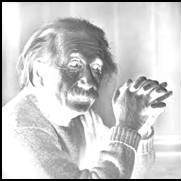
\includegraphics[scale = 0.67]{images/negative_out.png}}
\caption{After negative}
\label{fig:neg}
\end{figure}
\item \textit{Sharpening} : \\
We take the following image(Refer Figures (\ref{fig:sharp_1} and \ref{fig:sharp_2}):
     \begin{figure}[htbp]
\centerline{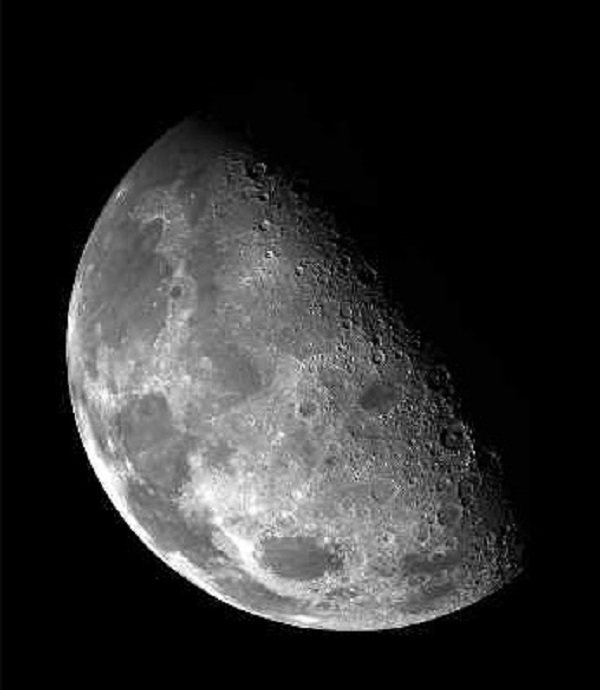
\includegraphics[scale = 0.30]{images/sharp.jpg}}
\caption{Before sharpening}
\label{fig:sharp_1}
\end{figure}
    \begin{figure}[htbp]
\centerline{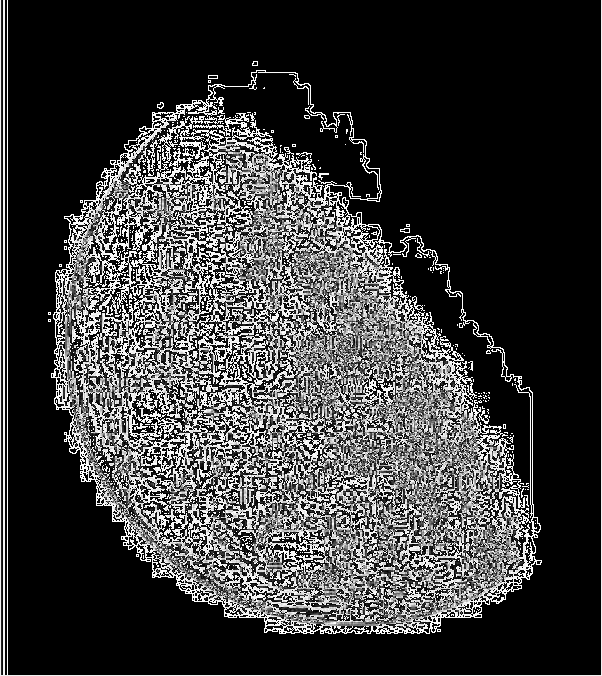
\includegraphics[scale = 0.30]{images/sharp_out.png}}
\caption{After Sharpening}
\label{fig:sharp_2}
\end{figure}

 \end{enumerate}

\section*{Conclusion and discussion}
The main challenges I faced was to implement the GUI which did end up taking  a lot of time since I was new to Tkinter in python. I was not able to complete many features like undo, undo-all and save in the GUI which I would like to complete. Given more time, I would have loved to play around with the images more and apply some range of parameters to the image transformations like gamma correct etc.

%\section*{References}

%Please number citations consecutively within brackets \cite{b1}. The 
%sentence punctuation follows the bracket \cite{b2}. Refer simply to the reference 
%number, as in \cite{b3}---do not use ``Ref. \cite{b3}'' or ``reference \cite{b3}'' except at 
%the beginning of a sentence: ``Reference \cite{b3} was the first $\ldots$''

%Number footnotes separately in superscripts. Place the actual footnote at 
%the bottom of the column in which it was cited. Do not put footnotes in the 
%abstract or reference list. Use letters for table footnotes.

%Unless there are six authors or more give all authors' names; do not use 
%``et al.''. Papers that have not been published, even if they have been 
%submitted for publication, should be cited as ``unpublished'' \cite{b4}. Papers 
%that have been accepted for publication should be cited as ``in press'' \cite{b5}. 
%Capitalize only the first word in a paper title, except for proper nouns and 
%element symbols.

%For papers published in translation journals, please give the English citation first, followed by the original foreign-language citation \cite{b6}.
\newpage
\begin{thebibliography}{00}
\bibitem{b1} \url{https://medium.com/@kyawsawhtoon/a-tutorial-to-histogram-equalization-497600f270e2}
\bibitem{b2} \url{Stackoverflow(for-general-doubts)}
\bibitem{b3} \url{https://towardsdatascience.com/histogram-equalization-a-simple-way-to-improve-the-contrast-of-your-image-bcd66596d815}
\bibitem{b4} \url{#https://numpy.org/doc/stable/reference/generated/numpy.pad.html}
\bibitem{b5} \url{https://www.cambridgeincolour.com/tutorials/gamma-correction.htm}
\bibitem{b6} \url{https://www.tutorialspoint.com/dip/gray_level_transformations.htm}
\bibitem{b7} \url{http://www.idlcoyote.com/ip_tips/sharpen.html}
%\bibitem{b6} Y. Yorozu, M. Hirano, K. Oka, and Y. Tagawa, ``Electron spectroscopy studies on magneto-optical media and plastic substrate interface,'' IEEE Transl. J. Magn. Japan, vol. 2, pp. 740--741, August 1987 [Digests 9th Annual Conf. Magnetics Japan, p. 301, 1982].
%\bibitem{b7} M. Young, The Technical Writer's Handbook. Mill Valley, CA: University Science, 1989.
\end{thebibliography}

\vspace{12pt}
% \color{red}
% IEEE conference templates contain guidance text for composing and formatting conference papers. Please ensure that all template text is removed from your conference paper prior to submission to the conference. Failure to remove the template text from your paper may result in your paper not being published.
}}
\end{document}
